In order to compute the dynamic topography we will need $\sigma_{rr}$, 
which in fact will require $\dot{\varepsilon}_{rr}$. This means that 
having obtained the strain rate tensor in Cartesian coordinates we must 
rewrite it in spherical coordinates with the following conventions:

\begin{center}
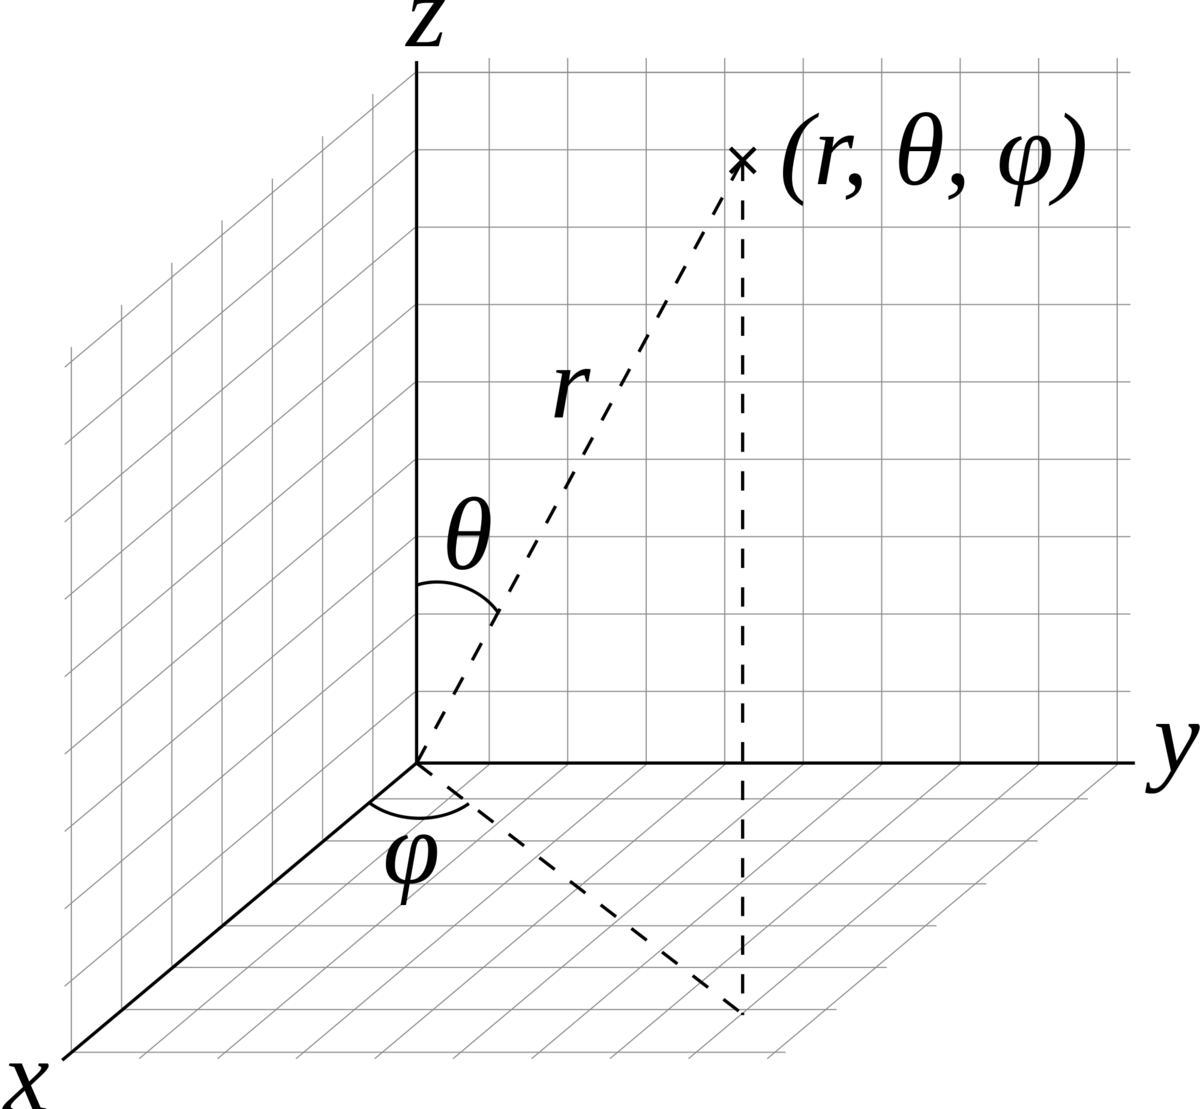
\includegraphics[width=3cm]{images/sphcoord}
\end{center}

We have
\begin{eqnarray}
{\bm T}_{\tiny Sph}&=&
\left(
\begin{array}{ccc}
T_{rr}       & T_{r\theta}      & T_{r\phi} \\
T_{\theta r} & T_{\theta\theta} & T_{\theta\phi} \\
T_{\phi r}   & T_{\phi \theta}  & T_{\phi\phi}
\end{array}
\right) \nn\\
&=&
\left(
\begin{array}{ccc}
\sin\theta \cos\phi & \sin\theta \sin\phi & \cos\theta \\
\cos\theta \cos\phi & \cos\theta \sin\phi & -\sin\theta \\
-\sin\phi & \cos\phi & 0 
\end{array}
\right)
\cdot
\left(
\begin{array}{ccc}
T_{xx} & T_{xy} & T_{xz} \\
T_{yx} & T_{yy} & T_{yz} \\
T_{zx} & T_{zy} & T_{zz} 
\end{array}
\right)
\cdot
\left(
\begin{array}{ccc}
\sin\theta\cos\phi & \cos\theta\cos\phi & -\sin\phi \\
\sin\theta\sin\phi & \cos\theta\sin\phi & \cos\phi \\
\cos\theta & -\sin\theta & 0
\end{array}
\right) 
\nn\\
{\bm T}_{\tiny Cart} &=&
\left(
\begin{array}{ccc}
T_{xx} & T_{xy} & T_{xz} \\
T_{yx} & T_{yy} & T_{yz} \\
T_{zx} & T_{zy} & T_{zz} 
\end{array}
\right) \nn\\
&=&
\left(
\begin{array}{ccc}
\sin\theta\cos\phi & \cos\theta\cos\phi & -\sin\phi \\
\sin\theta\sin\phi & \cos\theta\sin\phi & \cos\phi \\
\cos\theta & -\sin\theta & 0
\end{array}
\right)
\cdot
\left(
\begin{array}{ccc}
T_{rr}       & T_{r\theta}      & T_{r\phi} \\
T_{\theta r} & T_{\theta\theta} & T_{\theta\phi} \\
T_{\phi r}   & T_{\phi \theta}  & T_{\phi\phi}
\end{array}
\right)
\cdot
\left(
\begin{array}{ccc}
\sin\theta \cos\phi & \sin\theta \sin\phi & \cos\theta \\
\cos\theta \cos\phi & \cos\theta \sin\phi & -\sin\theta \\
-\sin\phi & \cos\phi & 0 
\end{array}
\right) \nonumber
\end{eqnarray}
In our case, calculations take place in the 
$(x,z)$-plane so we have $\phi=0$ and the equation above 
becomes
\[
\left(
\begin{array}{ccc}
T_{rr}       & T_{r\theta}      & T_{r\phi} \\
T_{\theta r} & T_{\theta\theta} & T_{\theta\phi} \\
T_{\phi r}   & T_{\phi \theta}  & T_{\phi\phi}
\end{array}
\right)
=
\left(
\begin{array}{ccc}
\sin\theta  & 0 & \cos\theta \\
\cos\theta  & 0 & -\sin\theta \\
0 & 1 & 0 
\end{array}
\right)
\cdot
\left(
\begin{array}{ccc}
T_{xx} & T_{xy} & T_{xz} \\
T_{yx} & T_{yy} & T_{yz} \\
T_{zx} & T_{zy} & T_{zz} 
\end{array}
\right)
\cdot
\left(
\begin{array}{ccc}
\sin\theta & \cos\theta & 0 \\
0 & 0 & 1 \\
\cos\theta & -\sin\theta & 0
\end{array}
\right)
\]
We define $c_\theta=\cos\theta$, $s_\theta=\sin\theta$ so that
\[
\left(
\begin{array}{ccc}
T_{rr}       & T_{r\theta}      & T_{r\phi} \\
T_{\theta r} & T_{\theta\theta} & T_{\theta\phi} \\
T_{\phi r}   & T_{\phi \theta}  & T_{\phi\phi}
\end{array}
\right)
=
\left(
\begin{array}{ccc}
s_\theta  & 0 & c_\theta \\
c_\theta  & 0 & -s_\theta \\
0 & 1 & 0 
\end{array}
\right)
\cdot
\left(
\begin{array}{ccc}
T_{xx} & T_{xy} & T_{xz} \\
T_{yx} & T_{yy} & T_{yz} \\
T_{zx} & T_{zy} & T_{zz} 
\end{array}
\right)
\cdot
\left(
\begin{array}{ccc}
s_\theta & c_\theta & 0 \\
0 & 0 & 1 \\
c_\theta & -s_\theta & 0
\end{array}
\right)
\]
As we have seen above we have 
\[
\dot{\bm\varepsilon}_{\tiny Cart}
=
\left(
\begin{array}{ccc}
\dot\varepsilon_{xx} & 0 & \dot{\varepsilon}_{xz} \\
0 & \dot{\varepsilon}_{yy}  & 0 \\
\dot{\varepsilon}_{xz} & 0 & \dot\varepsilon_{zz}
\end{array}
\right)
\]
so 
\begin{eqnarray}
\dot{\bm \varepsilon}_{\tiny Sph}=
\left(
\begin{array}{ccc}
\dot\varepsilon_{rr}       & \dot\varepsilon_{r\theta}      & \dot\varepsilon_{r\phi} \\
\dot\varepsilon_{\theta r} & \dot\varepsilon_{\theta\theta} & \dot\varepsilon_{\theta\phi} \\
\dot\varepsilon_{\phi r}   & \dot\varepsilon_{\phi \theta}  & \dot\varepsilon_{\phi\phi}
\end{array}
\right)
&=&
\left(
\begin{array}{ccc}
s_\theta  & 0 & c_\theta \\
c_\theta  & 0 & -s_\theta \\
0 & 1 & 0 
\end{array}
\right)
\cdot
\left(
\begin{array}{ccc}
\dot\varepsilon_{xx} & 0 & \dot{\varepsilon}_{xz} \\
0 & \dot{\varepsilon}_{yy}  & 0 \\
\dot{\varepsilon}_{xz} & 0 & \dot\varepsilon_{zz}
\end{array}
\right)
\cdot
\left(
\begin{array}{ccc}
s_\theta & c_\theta & 0 \\
0 & 0 & 1 \\
c_\theta & -s_\theta & 0
\end{array}
\right)  \nonumber\\
&=&
\left(
\begin{array}{ccc}
s_\theta  & 0 & c_\theta \\
c_\theta  & 0 & -s_\theta \\
0 & 1 & 0 
\end{array}
\right)
\cdot
\left(
\begin{array}{ccc}
\dot\varepsilon_{xx} s_\theta + 
\dot\varepsilon_{xz} c_\theta  & 
\dot\varepsilon_{xx} c_\theta - 
\dot\varepsilon_{xz} s_\theta  &
0 \\
0 & 0 & \dot{\varepsilon}_{yy}  
\\
\dot\varepsilon_{xz} s_\theta + 
\dot\varepsilon_{zz} c_\theta  &
\dot\varepsilon_{xz} c_\theta - 
\dot\varepsilon_{zz} s_\theta  &
0 
\end{array}
\right)  \nonumber\\
&=&
\left(
\begin{array}{ccc}
\dot\varepsilon_{xx} s_\theta^2 + 
2 \dot\varepsilon_{xz} c_\theta  s_\theta +
\dot\varepsilon_{zz} c_\theta ^2  
& 
\dot\varepsilon_{xx} c_\theta s_\theta - 
\dot\varepsilon_{xz} s_\theta^2  +
\dot\varepsilon_{xz} c_\theta^2 - 
\dot\varepsilon_{zz} s_\theta c_\theta 
& 0 \\ \\
\dot\varepsilon_{xx} s_\theta c_\theta+ 
\dot\varepsilon_{xz} c_\theta^2  -
\dot\varepsilon_{xz} s_\theta^2 -
\dot\varepsilon_{zz} c_\theta s_\theta 
&
\dot\varepsilon_{xx} c_\theta^2 - 
2\dot\varepsilon_{xz} s_\theta c_\theta +
\dot\varepsilon_{zz} s_\theta^2  
& 0 
\\ \\
0 & 0 & \dot{\varepsilon}_{yy} 
\end{array}
\right)  \nonumber
\end{eqnarray}
We can easily verify that the trace of this tensor is zero.

In the code we need to be careful and use {\python theta\_sph}:

\begin{center}
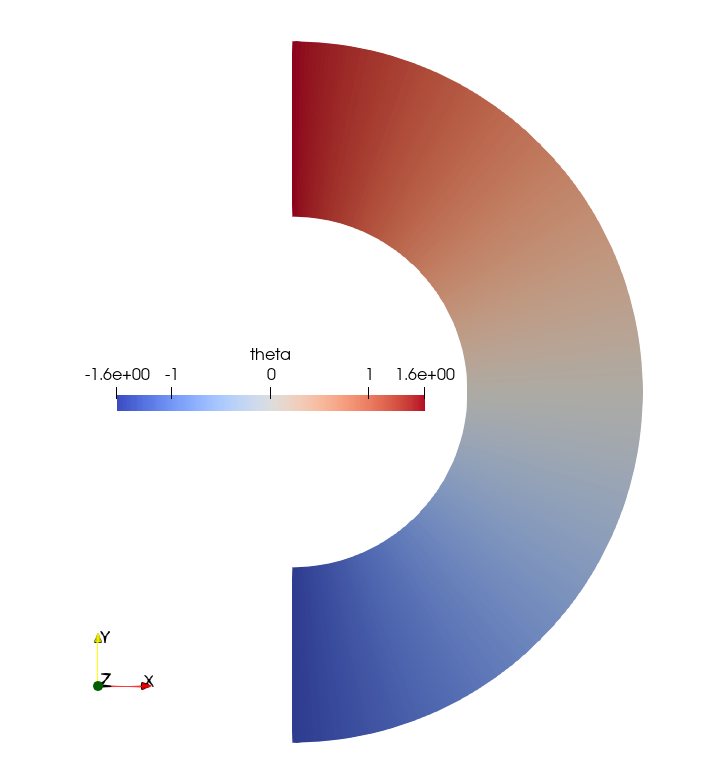
\includegraphics[width=8.3cm]{images/theta}
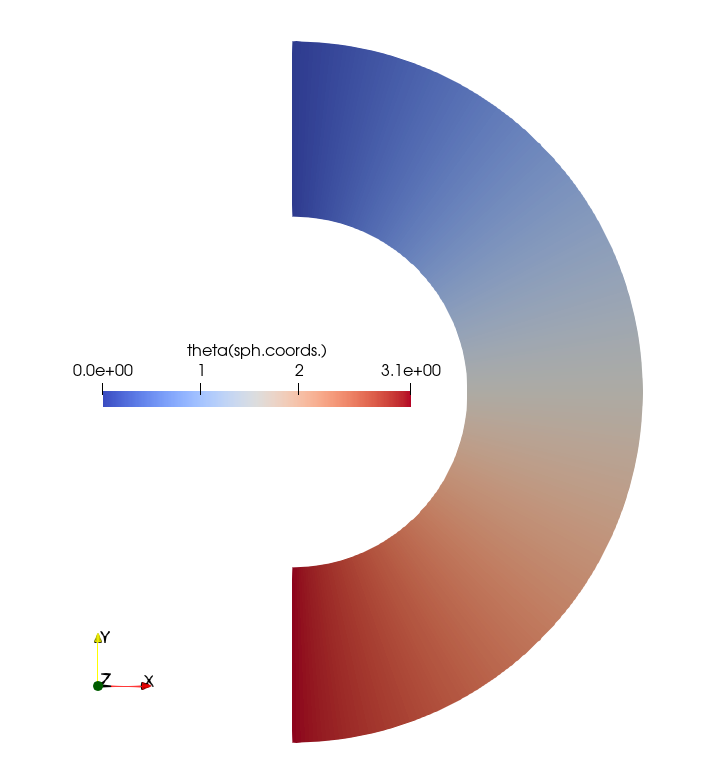
\includegraphics[width=8.3cm]{images/theta_sph}
\end{center}

\begin{lstlisting}
for i in range(0,NV):
    theta_sph[i]=np.pi/2-math.atan(yV[i]/abs(xV[i]))
    if xV[i]>=0:
       e_rr[i]=exx2[i]*np.sin(theta_sph[i])**2+\
               2*exy2[i]*np.sin(theta_sph[i])*np.cos(theta_sph[i])+\
               eyy2[i]*np.cos(theta_sph[i])**2
       e_tt[i]=exx2[i]*np.cos(theta_sph[i])**2-\
               2*exy2[i]*np.sin(theta_sph[i])*np.cos(theta_sph[i])+\
               eyy2[i]*np.sin(theta_sph[i])**2
       e_rt[i]=(exx2[i]-eyy2[i])*np.sin(theta_sph[i])*np.cos(theta_sph[i])+\
               exy2[i]*(-np.sin(theta_sph[i])**2+\
               np.cos(theta_sph[i])**2)
\end{lstlisting}



